\section{Compiler Verification}
\label{sec:intptrcast:compiler-verification}

In this section, we give a high-level overview of our reasoning principles
with a running example.

\subsection{Running Example \& Informal Verification}
\label{reasoning:running}

Consider the following example transformation, which is indeed
performed by ``clang -O2''.  This transformation involves four different optimizations: constant propagation (CP), dead load elimination
(DLE), dead store elimination (DSE), and dead allocation elimination
(DAE).
\begin{center}
\begin{tabular}{@{}l@{}l@{}l@{}}
%\small
\begin{lstlisting}
   foo(ptr p) {
     var ptr q, int a;
1:   q = malloc (1);
2:   *q = 123;
3:   bar(p);
4:   a = *q;
5:   *p = a;
   }
\end{lstlisting}
&
$\quad\rightarrow\quad$
&
%\small
\begin{lstlisting}
foo(ptr p) {

            // DAE
            // DSE
  bar(p);
            // DLE
  *p = 123; // CP
}
\end{lstlisting}
\end{tabular}
\end{center}

We will argue that at each line in the two versions of foo (source and target), the effects of the instruction executed (if any) are equivalent. To do so, we will assume an initial relationship between the memory of the source and target programs, and show that some variant of that relationship persists throughout the function, relying on any call to other functions to maintain a similar relationship. 

This relationship will designate one section of each memory as \emph{public}, and require that related locations in the source and target public memories have equivalent values; it will also designate a \emph{private} section of each memory, such that the source program can make changes to its private memory when the target does not make corresponding changes and vice versa. For the technical details of this relation and our notion of equivalence, see \S\ref{reasoning:invariants}.

\begin{figure}
\center
\begin{tabular}{l@{}l@{$\qquad\quad$}l@{}l}
\begin{minipage}{0.5cm}\vspace*{-.8cm}(a)\end{minipage} & 
\fbox{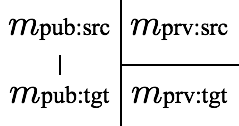
\includegraphics[height=1cm]{figure/memory-0.png}} &
\begin{minipage}{0.5cm}\vspace*{-.8cm}(b)\end{minipage} & 
\fbox{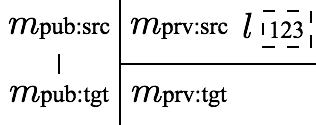
\includegraphics[height=1cm]{figure/memory-1.png}} \\[2mm]
\begin{minipage}{0.5cm}\vspace*{-.8cm}(c)\end{minipage} & 
\fbox{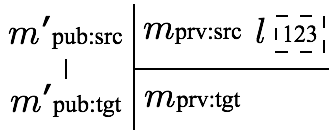
\includegraphics[height=1cm]{figure/memory-2.png}} &
\begin{minipage}{0.5cm}\vspace*{-.8cm}(d)\end{minipage} & 
\fbox{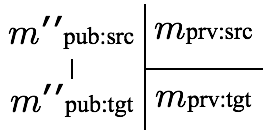
\includegraphics[height=1cm]{figure/memory-3.png}}
\end{tabular}
%
\caption{Memory Invariants for the Running Example}\label{fig:invex}
\end{figure}

We begin at line 1 by assuming the
following conditions on the memory of the source and target programs (see Figure~\ref{fig:invex}~(a)):
\begin{description}
\item[assume] (equivalent arguments) the parameter \texttt{p} contains
  \emph{equivalent} arguments $v_\textrm{src} $ in the source and $v_\textrm{tgt}$ in the target;
\item[assume] (equivalent public memories) 
  there are a set of memory blocks
  $m_\textrm{pub:src}$ in the source and
  $m_\textrm{pub:tgt}$ in the target that are
  \emph{equivalent} and publicly accessible by arbitrary functions;
\item[assume] (source private memory) 
  there is a disjoint set of blocks
  $m_\textrm{prv:src}$ in the source, each of which is
  exclusively owned by a single function;
\item[assume] (target private memory) 
  there is a disjoint set of blocks
  $m_\textrm{prv:tgt}$ in the target, each of which is
  exclusively owned by a single function.
\end{description}
After executing line 1, we add the newly allocated block (call it~$l$) to
the private source memory $m_\textrm{prv:src}$. It is important to note that we can add the
block $l$ to the private source memory because it is a fresh logical
block and thus exclusively owned by \texttt{foo}.  After executing
line 2, the block $l$ contains $123$ (see Figure~\ref{fig:invex}~(b)).

At line 3, we guarantee that the function calls to \texttt{bar} are
\emph{equivalent} as follows:
\begin{description}
\item[guarantee] (equivalent arguments) 
  the arguments $v_\textrm{src}$ and $v_\textrm{tgt}$ to \texttt{bar} are equivalent; 
\item[guarantee] (equivalent public memories) 
  $m_\textrm{pub:src}$ and $m_\textrm{pub:tgt}$,
  which are equivalent and publicly accessible;
\item[guarantee] (source private memory) 
  each location in $m_\textrm{prv:src} \uplus {[l\mapsto 123]}$,
  is exclusively owned by a single function;
\item[guarantee] (target private memory) 
  each location in $m_\textrm{prv:tgt}$
  is exclusively owned by a single function.
\end{description}
%After the calls to \texttt{bar}, 
When the calls to \texttt{bar} return,
we can assume that the new public
memories are equivalent to each other (though they may not be the same as the previous public memories), and
the private memories are untouched (see Figure~\ref{fig:invex}~(c)):
\begin{description}
\item[assume] (equivalent public memories) we have new public memories $m'_\textrm{pub:src}$ and
  $m'_\textrm{pub:tgt}$, which are \emph{evolved} from $m_\textrm{pub:src}$
  and $m_\textrm{pub:tgt}$ (see \S\ref{reasoning:simulation} for the definition of memory evolution), and 
  are equivalent and publicly accessible;
\item[assume] (source private memory) $m_\textrm{prv:src} \uplus
  {[l\mapsto 123]}$ is unchanged;
\item[assume] (target private memory) $m_\textrm{prv:tgt}$ is
  unchanged.
\end{description}

At line 4, we load the value $123$ from the source's private memory and
store it in the variable \texttt{a}.  At line 5, in the source, we
store the value of \texttt{a}, which is $123$, in the memory cell located at
the address $v_\texttt{src}$.  In the target, we store the constant
$123$ in the cell at $v_\texttt{tgt}$. Since we stored equivalent
values at equivalent locations $v_\texttt{src}$ and $v_\texttt{tgt}$,
we will have equivalent public memories $m''_\textrm{pub:src}$ and
$m''_\textrm{pub:tgt}$, while leaving the private memories unchanged.

Finally, we return to the callers of \texttt{foo} with (see Figure~\ref{fig:invex}~(d))
\begin{description}
\item[guarantee] (equivalent public memories) 
  $m''_\textrm{pub:src}$ and $m''_\textrm{pub:tgt}$
  that are evolved from $m_\textrm{pub:src}$ and $m_\textrm{pub:tgt}$,
  and are equivalent and publicly accessible;
\item[guarantee] (source private memory) 
  $m_\textrm{prv:src}$;
\item[guarantee] (target private memory) 
  $m_\textrm{prv:tgt}$,
\end{description}
where we can ignore the block $l$ because it is not going to be used any more.
Note that we here guarantee \text{foo} returns with the same private memories it was given
initially, as we assumed the same property for the function
\texttt{bar} after line 3.

\subsection{Memory Invariants}
\label{reasoning:invariants}

As informally discussed above, we prove program refinement using a memory invariant that places conditions on
public memories (which must be equivalent in the source and target programs) and private memories (which can differ between them).  We now formally define the
notion of memory equivalence used in our informal
example, and the conditions on the private memories.

The idea of memory equivalence is a simplification of CompCert's
memory injection \cite{Leroy-Appel-Blazy-Stewart-memory-v2}.  Our
conditions for concrete blocks are inspired from CompCertTSO's support
for finite memory \cite{vsevvcik2013compcerttso}.  See
\S\ref{sec:discussion} for more comparisons.

%%  in the source and the
%% target are exactly the same because optimizations like DAE may remove
%% memory blocks. Thus, we introduce a more relaxed notion of
%% equivalence.

\paragraph{Memory Equivalence}
We define a more relaxed notion of equivalence than simple equality,
which would be too strong in the presence of (unrelated) private
memories. We say that a set of blocks $m_\textrm{src}$ in the source
is equivalent to a set of blocks $m_\textrm{tgt}$ in the target
when they satisfy the following conditions. First, there should be a
bijection, say $\alpha$, between the block identifiers in
$m_\textrm{src}$ and those in $m_\textrm{tgt}$. Second, corresponding
blocks (\ie those related by $\alpha$) should have the same
size and validity, and the values they hold at each offset should be \emph{equivalent}.  Values are
equivalent (w.r.t. $\alpha$) when either both are the same integer, or
they are logical addresses that are at the same offset in corresponding blocks
(w.r.t.~$\alpha$). When $m_\textrm{src}$ and $m_\textrm{tgt}$ are equivalent in this sense, we write $m_\textrm{src} \simeq_\alpha m_\textrm{tgt}$.

\begin{figure}[t]
\center
  %% \fbox{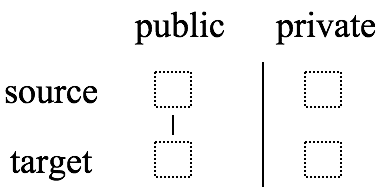
\includegraphics[scale=0.25]{figure/relation-compcert.png}}
  \begin{minipage}[b]{0.28\textwidth}
  \fbox{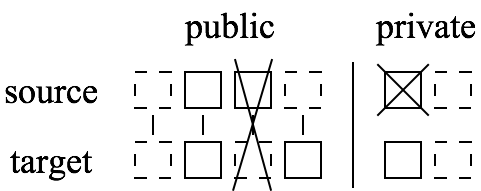
\includegraphics[scale=0.25]{figure/relation.png}}
  \end{minipage}
  \begin{minipage}[b]{0.14\textwidth}
  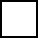
\includegraphics[scale=0.25]{figure/physical-block.png} concrete block\\[2mm]
  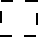
\includegraphics[scale=0.25]{figure/logical-block.png} logical block\\
  \mbox{}
  \end{minipage}
%% (1) for CompCert model, and (2) for our model
\caption{Memory Invariants for Quasi-Concrete Model}\label{fig:invariant}
\end{figure}

The condition on the concrete addresses of corresponding blocks
merits further explanation. We have four possible cases
regarding whether two corresponding blocks are concrete or logical (see the
\emph{public} side of Figure~\ref{fig:invariant}).  The first case in
the figure (\ie source: logical, target: logical) obviously should be
allowed. The second case (\ie source: concrete, target: concrete)
should also be allowed but only when the concrete addresses
coincide. 

The third case (\ie source: concrete, target: logical) should not be
allowed. To allow this case would be to allow the source memory to contain more concrete
blocks than the target, which leads to two problems: $(i)$ an arbitrary
concrete memory access may succeed in the source but fail in the
target; and $(ii)$ a pointer-to-integer cast may raise out-of-memory
in the source but succeed in the target.  In both cases, the target
may have more behaviors than the source, which is disallowed.  On the
other hand, the final case (\ie source: logical, target: concrete) is
allowed because the situation is exactly the opposite: the source may
have more behaviors than the target, which is allowed.

\paragraph{Private Memory}
For blocks in private memories, we have four possible cases
regarding whether the block is in the source or the target, and
whether the block is concrete or logical (see \emph{private} side of
Figure~\ref{fig:invariant}).  All the cases are allowed except for
source private memory blocks that are concrete, for the same reason
that blocks that are concrete in the source and logical in the target are not
allowed in memory equivalence: the source memory should not contain
more concrete blocks than the target memory.

\paragraph{Memory Invariants}
A memory invariant $\beta$ consists of $(i)$ a bijection $\alpha$ between their
block identifiers, $(ii)$ the source's private memory
$m_\textrm{prv:src}$, and $(iii)$ the target's private memory
$m_\textrm{prv:tgt}$. 
%% Recall that we call two memories equivalent when
%% their public sections are equivalent up to the bijection between block
%% identifiers. 
An invariant $\beta=(\alpha, m_\textrm{prv:src}, m_\textrm{prv:tgt})$ 
holds on a pair of memories $m_{\textrm{src}}$ and
$m_{\textrm{tgt}}$ when they contain the private sections $m_\textrm{prv:src}$ and 
$m_\textrm{prv:tgt}$
and some public sections $m_\textrm{pub:src}$ and
$m_\textrm{pub:tgt}$ such that:
%% their public sections
%% are equivalent and they contain the private sections of the
%% invariant. 
%% Formally, memories $m_{\textrm{src}}$ and
%% $m_{\textrm{tgt}}$ are related by a memory invariant $\beta=(\alpha,
%% m_\textrm{prv:src}, m_\textrm{prv:tgt})$ if there exist 
%% public sections $m_\textrm{pub:src}$ and $m_\textrm{pub:tgt}$ that are equivalent 
%% w.r.t.~$\alpha$
  \[\begin{array}{@{}l}
    (m_{\textrm{src}} \supseteq m_\textrm{pub:src} \uplus m_\textrm{prv:src})~\land~
    (m_{\textrm{tgt}} \supseteq m_\textrm{pub:tgt} \uplus m_\textrm{prv:tgt})~\land\\m_{\textrm{pub:src}} \simeq_\alpha m_{\textrm{pub:tgt}}
  \end{array}\]
  where 
%$\equiv_\alpha$ is the equivalence w.r.t. $\alpha$, and 
$\uplus$ and $\subseteq$ are the disjoint union and the subset relation.

\subsection{Proving Simulation}
\label{reasoning:simulation}

We are now ready to present our reasoning principle formally. Our
basic approach is to verify programs via local simulation in the style
of \cite{Hur:2012:MBK:2103656.2103666}.

%\newcommand{\assumedinvariant}[1]{\widehat{#1}}

A function, say \texttt{foo}, in the source and target is locally
simulated if it satisfies the following conditions.  First, consider
a typical lifecycle of the source and target functions:
\begin{center}
\begin{minipage}{0.475\textwidth}
\begin{lstlisting}
foo(|..|) {        foo(|..|) {  //|\fbox{${\beta_\text{s}}$}|
  ...              ...      //|\hspace*{3pt}$\beta_\text{c}\quad{\beta_\text{s}}\!\sqsubseteq\!\beta_\text{c}$|
  bar(..);         bar(..); //|\fbox{${\beta_\text{r}}\quad\beta_\text{c}\!\sqsubseteq\!{\beta_\text{r}} \,\land\, \beta_\text{c}\!=_{\textrm{prv}}\!{\beta_\text{r}}$}|
  ...        $\rightarrow$    ...      //|\hspace*{3pt}$\beta'_\text{c}\quad{\beta_\text{r}}\!\sqsubseteq\!\beta'_\text{c}$|
  gee(..);         gee(..); //|\fbox{${\beta'_\text{r}}\quad\beta'_\text{c}\!\sqsubseteq\!{\beta'_\text{r}} \,\land\, \beta'_\text{c}\!=_{\textrm{prv}}\!{\beta'_\text{r}}$}|
  ...              ...      //|\hspace*{3pt}$\beta_\text{e}\quad{\beta'_\text{r}}\!\sqsubseteq\!\beta_\text{e} \;\land\; {\beta_\text{s}}\!=_{\textrm{prv}}\!\beta_\text{e}$|
}                }
\end{lstlisting}
\end{minipage}
\end{center}
Here boxed conditions are assumed and the others are guaranteed.

First, in \texttt{foo}, unknown functional calls such as
\texttt{bar(..)} and \texttt{gee(..)} should be synchronized (\ie when
the target calls \texttt{bar}, the source should call \texttt{bar} as
well). Note that when a known function is called, the verifier can either step into
the called function and reason about its code, or treat
it as an unknown function call.

Next, at the entry point of \texttt{foo}, we assume that we are given
memories satisfying a given invariant $\beta_\textrm{s}$, and
equivalent arguments w.r.t. the bijection in $\beta_\textrm{s}$.
Then, we execute the code of \textrm{foo} in the source and the target
until the first unknown function call to \texttt{bar(..)}.  Here we have
to show that there is some invariant $\beta_\textrm{c}$ that holds on
the current memories and that the arguments to the function \texttt{bar}
are equivalent w.r.t. the bijection in $\beta_\textrm{c}$.

Here, we also have to show that the current memories are
\emph{evolved} from the memories given initially by showing that the
current invariant $\beta_\textrm{c}$ is a \emph{future invariant} of
the initial one ${\beta_\textrm{s}}$ 
(denoted ${\beta_\textrm{s}}\sqsubseteq\beta_\textrm{c}$).
We say that $\beta_\textrm{c}$ is a future invariant of 
${\beta_\textrm{s}}$ when satisfying the following conditions,
which rule out changes to the memory that cannot be caused 
by the language's operational semantics.  
%% This invariant $\beta_\textrm{c}$ must also be a \emph{future invariant}
%% of ${\beta_\textrm{s}}$ (denoted ${\beta_\textrm{s}}\sqsubseteq\beta_\textrm{c}$), 
%% which rules out changes to the memory that cannot be caused by the language's operational semantics.  
%% More precisely, 
First, the bijection in
$\beta_\textrm{c}$ should include the bijection of ${\beta_\textrm{s}}$ because
logical blocks cannot be removed during execution (a block
becomes invalid rather than removed when it is freed).  Second, the other
conditions on the public memories in ${\beta_\textrm{s}}$ and
$\beta_\textrm{c}$ are that $(i)$ the size of a block does not change
between ${\beta_\textrm{s}}$ and $\beta_\textrm{c}$, $(ii)$ an
invalid block in ${\beta_\textrm{s}}$ cannot become valid in
$\beta_\textrm{c}$, and $(iii)$ a concrete block in
${\beta_\textrm{s}}$ cannot become logical in $\beta_\textrm{c}$.
However, it is important to note that the contents of public memories
can change between ${\beta_\textrm{s}}$ and $\beta_\textrm{c}$ because
the operational semantics allows
%the called function 
to update values in memory.

Then, we consider the case when the unknown function successfully
returns. We can assume that the memories at return time also satisfy some
\emph{future} invariant ${\beta_\textrm{r}}$. We can also
assume that the function \texttt{bar} does not change the private
memories in $\beta_\textrm{c}$ (denoted $\beta_\textrm{c}
=_{\textrm{prv}} {\beta_\textrm{r}}$) because there is no way
for \texttt{bar} to access them in our quasi-concrete model.

We continue through the function, evolving our invariant at non-call steps and performing similar reasoning at other call sites
such as $\texttt{gee(..)}$.  Finally, when \texttt{foo} returns to its caller, we have to
show that there is some \emph{future} invariant $\beta_\textrm{e}$
that holds on the current memories. Furthermore, we have to show that
we did not change the private memories given in
 the initial invariant $\beta_\textrm{s}$ (\ie $\beta_\textrm{s} =_{\textrm{prv}}
\beta_\textrm{e}$). This condition is necessary because, as seen above, we assume that this property holds at the end of any other function call.
In this way, we construct a local simulation proof for the $\texttt{foo}$.


\subsection{Examples}
\label{sec:intptrcast:compiler-verification:examples}

In this section, we show how to verify the examples shown in \S\ref{sec:quasi}.  All
results here are fully formalized in Coq.

\paragraph{Arithmetic Optimization I}

Consider the transformation in Figure~\ref{code:arith1}. If we assume that integer variables only contain integer
values, not logical addresses, the instruction \texttt{a = (a
  - b) + (2 * b - b)} has no effect on the value of \texttt{a} and is equivalent to no
operation, so the optimization is trivially correct. 

How do we know that integer variables only contain
integer values? The straightforward answer is that our language is statically type-checked, as in the LLVM IR. However, the key reason why this is possible
is that in the quasi-concrete model we actually turn logical addresses into integers
when they are cast to \texttt{int}, rather than placing logical addresses in integer
variables. Also, when we load a value from memory to an integer 
variable (resp. a pointer variable), 
if the loaded value is a logical address (resp. an integer value), we raise undefined
behavior (\ie \emph{error}).
In other words, the quasi-concrete model induces a form of dynamic type
checking in languages that use it. This allows us to verify integer
arithmetic optimizations as in this example.
%% and is only a minor
%% inconvenience to the user. If a programmer using the model wants to
%% load a value whose type is unknown, she can load that value to a
%% pointer-type variable (equivalent to a (void *)-type variable in C)
%% and cast it to whatever type she wants.  Since the pointer type
%% contains both integer values and logical addresses, a load to a
%% pointer-type variable will always succeed.

\paragraph{Dead Code Elimination}

Consider the transformation in Figure~\ref{code:dce}.  This example
is similar to the previous one.  Since we can assume that integer-typed
variables contain only integers, the execution of the call
\texttt{foo(a)} does not have any side effects.
Furthermore, because we know the code of the function
\texttt{foo}, we do not need to treat it as an unknown function call.
Rather, we just step into the code of the function \texttt{foo} and
execute it in the source.%  In this way, we can easily verify this
% transformation.

\paragraph{Ownership Transfer}

Consider the transformation in Figure~\ref{code:ownership}.  This
example is similar to the running example in
\S\ref{reasoning:running}.

Assume that the first invariant below holds before the \texttt{malloc}.  After
allocating blocks $l_\text{s}$ in the source and $l_\text{t}$ in
the target, and storing 123 in both blocks, we can move the blocks $l_\text{s}$
and $l_\text{t}$ into the private sections of the invariant because they are logical and disjoint from the
public sections, yielding the second invariant below. Next we call the function \texttt{bar}. When it
returns, we can assume that the third invariant holds (\ie the
private sections are untouched). After loading, the variable
\texttt{a} will contain 123, since \texttt{p} contains the
logical address $(l_\text{s},0)$ in the source and $(l_\text{t},0)$ in
the target. 

Next, when we call \texttt{hash\_put}, we have to make sure that the
arguments are equivalent. The first arguments are equivalent because
we assume that we start with equivalent values in variables, and the third arguments
are equivalent because \texttt{a} contains 123.  To show that
the second arguments, $(l_\text{s},0)$ and $(l_\text{t},0)$, are
equivalent, we move the blocks from the private sections to the public
section and extend the bijection $\alpha'$ to relate $l_\text{s}$
and $l_\text{t})$ (the fourth invariant below). Such ownership
transfer from the private sections to the public section is allowed
because the future invariant relation ($\sqsubseteq$) requires
only the bijection to be non-decreasing, not the private
sections.
\begin{center}
\fbox{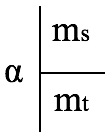
\includegraphics[scale=0.25]{figure/ownership-0.png}}\hfill
\fbox{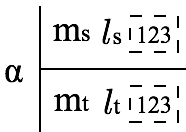
\includegraphics[scale=0.25]{figure/ownership-1.png}}\hfill
\fbox{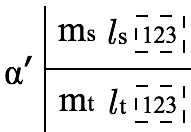
\includegraphics[scale=0.25]{figure/ownership-2.png}}\hfill
\fbox{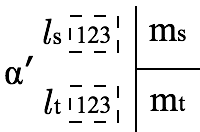
\includegraphics[scale=0.25]{figure/ownership-3.png}}
\end{center}

% \begin{lstlisting}
% foo(int i) {
%   var ptr p, ptr q, int r;
%   p = malloc (1);
%   q = malloc (10);
%   3 -> p;
%   5 -> q + i;
%   bar();
%   r <- p;
%   goo(r, (int) p);     $\to$ goo(3, (int) p);
% }
% \end{lstlisting}

% \begin{itemize}
% \item \texttt{p} is known to contain \texttt{3}, so we replace a use
%   of \texttt{r} by \texttt{3}.
% \item We can perform constant propagation optimization to this example
%   even though 1) there is a store to another block (\texttt{q})
%   between the store to and the load from \texttt{p}, 2) there is an
%   function call to an unknown function \texttt{bar} between the store
%   and the load, and 3) the exclusive ownership of \texttt{p} is lost
%   after the load from \text{p}.  Since \texttt{p} is allocated as a
%   logical block, can mark \texttt{p} as private.  Thus \texttt{r}
%   should be \texttt{3} after the function call to \texttt{bar}.
% \item If a pointer is determinted to be physical or logical at the
%   allocation time, this example is not justified due to ownership
%   transfer.  Since \texttt{p} is casted to integer, it should be
%   allocated at a physical address.  Thus \texttt{p} should be marked
%   as public, and \texttt{bar} may modify the content of \texttt{p}.
% \end{itemize}


\paragraph{Arithmetic Optimization II}

We can easily verify the transformation in Figure~\ref{code:arith2}
for the same reason as in \S\ref{ex:arith1}: because we can assume
that all integer variables contain integer values.

% \begin{itemize}
% \item Thanks to elaboration, we know the type of operands of every
%   operation.  For example, we can distinguish integer additions based
%   on the type of operands ($\texttt{+}_{\mathtt{ii}}$ between two
%   integers, $\texttt{+}_{\mathtt{pi}}$ between a pointer and an
%   integer, and $\texttt{+}_{\mathtt{ip}}$ between an integer and a
%   pointer).
% \item Standard integer optimizations are justified in our model, as
%   integer variables really contain integer values, not logical
%   pointers.  For instance, the above optimization is justified in our
%   model: the source program that require 4 integer operations into the
%   target program that require 3 integer operations.
% \item However, this optimization is not justified in the CompCert
%   model.  Suppose \texttt{a} contains an integer, and \texttt{b0},
%   \texttt{b1} and \texttt{b2} contain logical pointers of the same
%   block.  Since \texttt{a - b0} is \texttt{Vundef}, the operands of
%   two \texttt{printf}'s in the target are unconstrained, while those
%   of the source are specific integers.
% \end{itemize}

\paragraph{Dead Cast Elimination}

Consider the transformation in Figure~\ref{code:deadcast}, in the case in which
the source uses the quasi-concrete model and the target uses the
concrete model.

We begin by assuming that the first invariant below holds before the call to
\texttt{foo}, where the variable \texttt{p} contains equivalent
addresses $(l_\text{s},i)$ in the source and $\toint{(l_\text{t},i)}{m}$ in the target.
Note that the block $l_\text{t}$ is concrete, since the target is using
the fully concrete model. After the allocation of a block, say
$l'_\text{s}$, in \texttt{foo} in the source, we move it to the source's
private memory, yielding the second invariant below.  Here it is important
to note that if the source was using the concrete model, we could not move
the block $l'_\text{s}$ into the private section because $l'_\text{s}$
would be concrete, which would invalidate our proof.

After the cast, the block $l_\text{s}$ becomes concrete, yielding the third
invariant below.  Here it is important to note that if the target
language was using the quasi-concrete model and $l_\text{t}$ were logical,
then we would produce an invariant in which $l_\text{s}$ is
concrete and $l_\text{t}$ is logical, which would be an invalid invariant.  After
\texttt{foo} returns, we simply drop the block $l'_\text{s}$ from the
source private section because we do not use it, yielding the fourth
invariant below. Then we can proceed to verify the rest of the code.
\[
\fbox{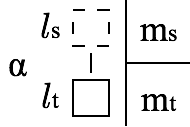
\includegraphics[height=.95cm]{figure/deadcast-0.png}}\,
\fbox{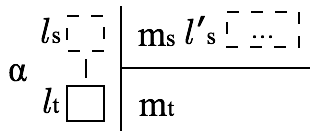
\includegraphics[height=.95cm]{figure/deadcast-1.png}}\,
\fbox{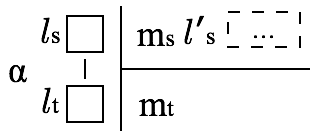
\includegraphics[height=.95cm]{figure/deadcast-2.png}}\,
\fbox{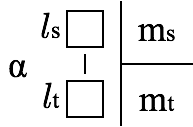
\includegraphics[height=.95cm]{figure/deadcast-3.png}}
\]

\paragraph{Identity Compilers}
As a sanity check for our reasoning principles, we wrote an identity compiler from our language with the quasi-concrete
model to itself, and a simple compiler from our language with the quasi-concrete
model to the same language with the concrete model. The latter compiler just eliminates
dead casts of the form ${\texttt{\_ = (int) p}}$. We successfully verified these two compilers in Coq using our reasoning principles.

% \begin{tabular}{ll}
% \small
% \begin{lstlisting}
% foo(int i) {
%   var ptr p, int r;
%   p = malloc (10);
%   3 -> p + i;
%   bar();
%   r <- p + i;
%   free (p);
% }
% \end{lstlisting}
% \begin{lstlisting}
% foo(int i) {



%   bar();


% }
% \end{lstlisting}
% \end{tabular}

% \begin{itemize}
% \item If a block is not physically realized, then we can optimize as
%   in the logical model.  In the above example, we can optimize out
%   everything related to the memory block allocated at \texttt{p}.
% \end{itemize}

% \begin{tabular}{ll}
% \begin{lstlisting}
% foo(ptr p) {
%   var int i;
%   i = (int) p;
%   bar(i);
% }
% \end{lstlisting}
% \begin{lstlisting}
% bar(int i) {
%   var int j;
%   j = i * 3;   $\to$ skip
% }
% \end{lstlisting}
% \end{tabular}

% \begin{itemize}
% \item In our model, this example is justified.  Since casting to
%   integer requires pointers to take physical address, \texttt{i}
%   contains an integer, not a logical pointer.  Thus we can optimize
%   out the multiplication without worrying about side effects.
% \item In the CompCert model, casts between integers and pointers are
%   ignored, and integer variables may contain logical pointer values.
%   When an operation require an integer but a logical pointer is given,
%   CompCert return \texttt{Vundef} (undefined value). 
% \item \todo{What is the point of this example?}
% \end{itemize}


%%% Local Variables:
%%% mode: latex
%%% TeX-master: "main"
%%% TeX-command-extra-options: "-shell-escape"
%%% End:
